\documentclass[12pt]{article}

\usepackage[russian]{babel}

\usepackage[letterpaper,top=2cm,bottom=2cm,left=3cm,right=3cm,marginparwidth=1.75cm]{geometry}

\usepackage{amsmath}
\usepackage{amssymb}
\usepackage{graphicx}
\usepackage[colorlinks=true, allcolors=blue]{hyperref}
\usepackage{float}
\usepackage{trfsigns}

\begin{document}
	\begin{center}
		\Large \textbf{Компьютерное управление скоростью вращения вала электромотора}
	\end{center}
	
	\section{Построение математической модели}
	\subsection{Принцип работы электродвигателя}
	\quad
	Объектом управления в данной работе является двигатель постоянного тока. Цель управления - поддержание заданной скорости вращения вала.\\
	Рассмотрим проводящий контур сопротивлением $R_s$, к которому приложена разность потенциалов $V_m$. Постоянный электрический ток $I_s$ создает магнитное поле. Согласно закону Био-Савара-Лапласа, 
	\begin{equation}
		\vec{B}(\vec{r_0})=\dfrac{\mu_0}{4\pi}\int_{\gamma}\dfrac{I_s[d\vec{r}\times (\vec{r_0}-\vec{r})]}{||\vec{r_0}-\vec{r}||^3},
	\end{equation}
	где $\mu_0$ - магнитная постоянная. Рассматриваемый контур является неподвижным и, как правило, представлет собой соленоид. Для соленоида с числом витков $n$ поле однородно и направлено вдоль оси (рис. 1): 
	\begin{equation}
		B=\mu_0nI_s.
	\end{equation}
	В электродвигателе соленоид служит статором.
	
	\begin{figure}[H]
		\centering
		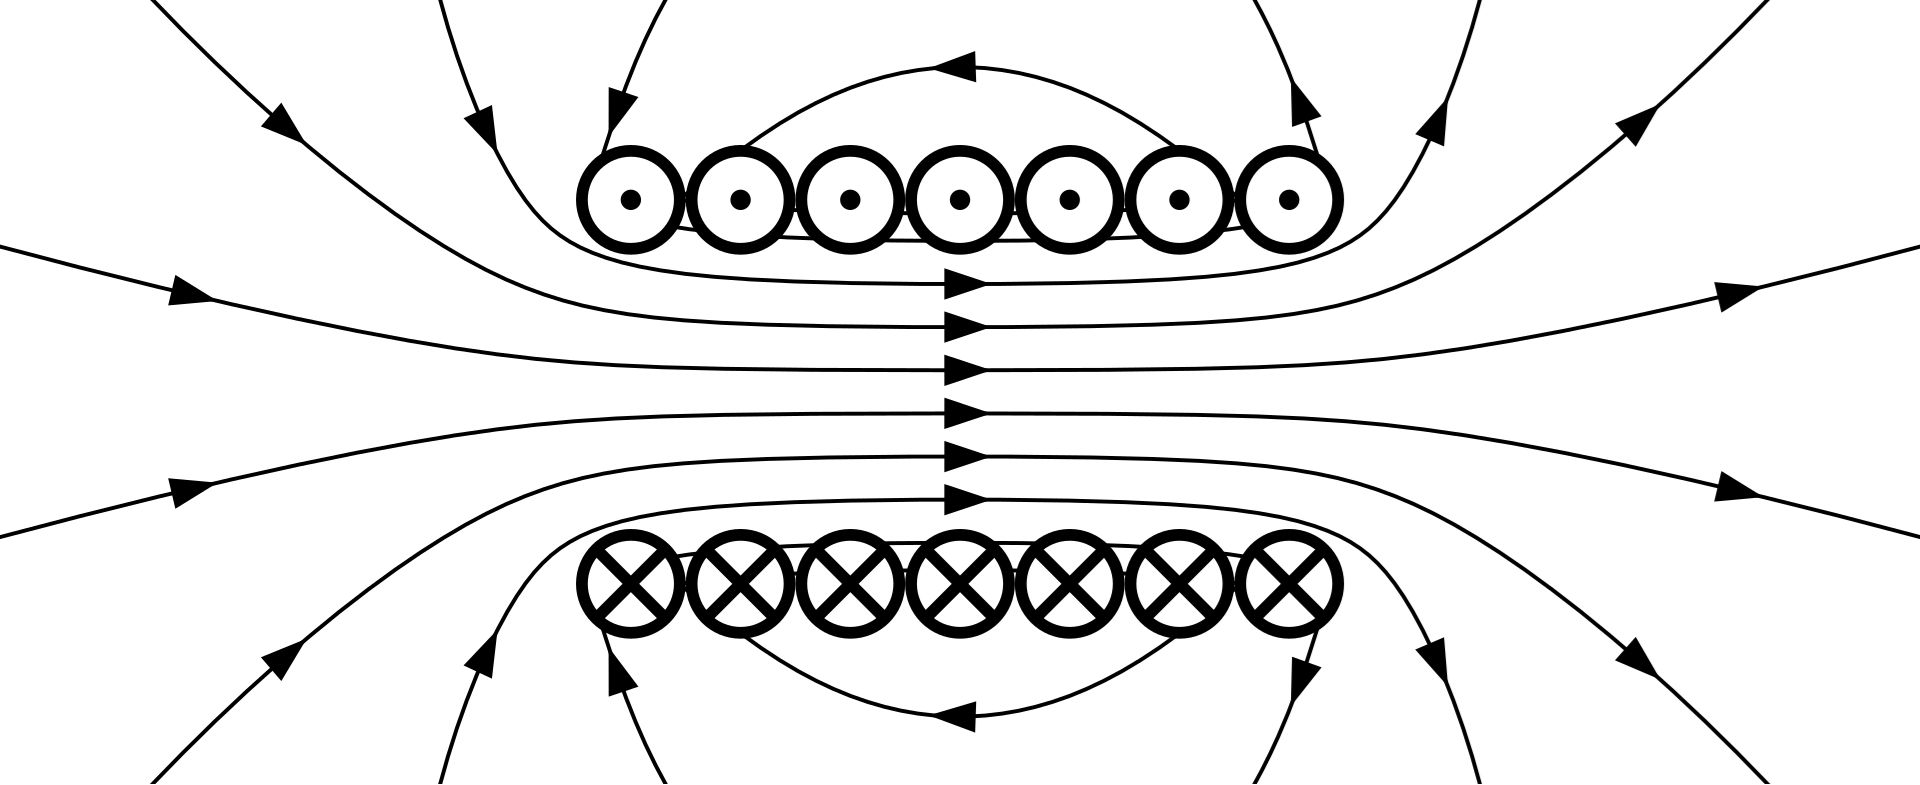
\includegraphics[scale=0.3]{Solenoid.png}
		\caption{\label{fig:Solenoid}Образование магнитного потока в соленоиде.}
	\end{figure}
	
	Поместим в магнитное поле проводящую рамку, подключив ее параллельно статору (рис. 2). В рамке сопротивлением $R_m$ течет постоянный ток $I_m$. В предполощении достаточной тонкости проводника действующую на рамку силу Ампера можно представить как 
	\begin{equation}
		\vec{F}=\oint_{l}I_md\vec{l}\times \vec{B}.
	\end{equation}
	Сила Ампера создает вращающий момент. Максимальный момент достигается, когда плоскость рамки параллельная полю (нормаль ортогональна $\vec{B}$). В этом случае
	\begin{equation}
		M_m=K_mI_m,
	\end{equation}
	где $K_m=2aLB$ (здесь $a$ - расстояние от оси вращения до стороны рамки, $L$ - длина стороны). В электродвигателе рассмотренная рамка конструктивно является ротором.
	
	\begin{figure}[H]
		\centering
		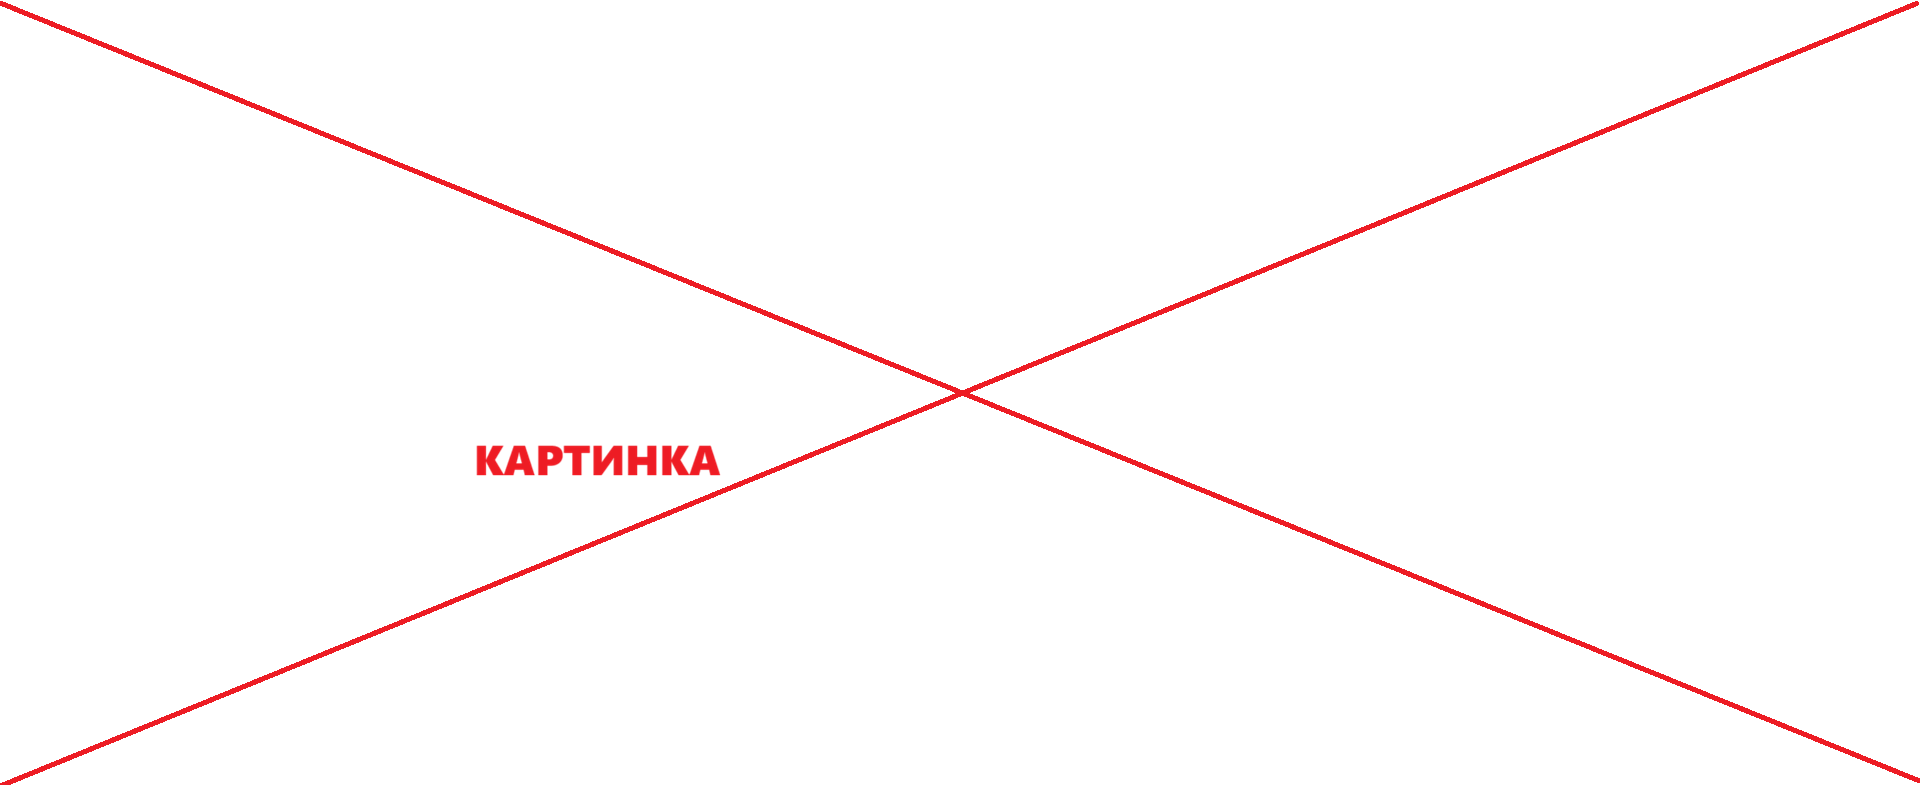
\includegraphics[scale=0.3]{template.png}
		\caption{\label{fig:template}Картинка однорамочного двигателя.}
	\end{figure}
	
	Спроектированная конструкция имеет существенный недостаток: в один из моментов перпендикулярности плоскости рамки линиям магнитной индукции $\vec{B}$ (т.н. нейтральное положение) вращение полностью прекратится. Для непрерывного вращения используется коллектор, переключающий ток в рамке при прохождении нейтральных положений. Контакт с пластинами коллектора обеспечивают прижимные щетки. Такая конструкция способна к непрерывному неравномерному вращению с замеделением вблизи нейтральных положений. Для обеспечения равномерного вращения используются многорамочные электродвигатели (рис. 3).
	
	\begin{figure}[H]
		\centering
		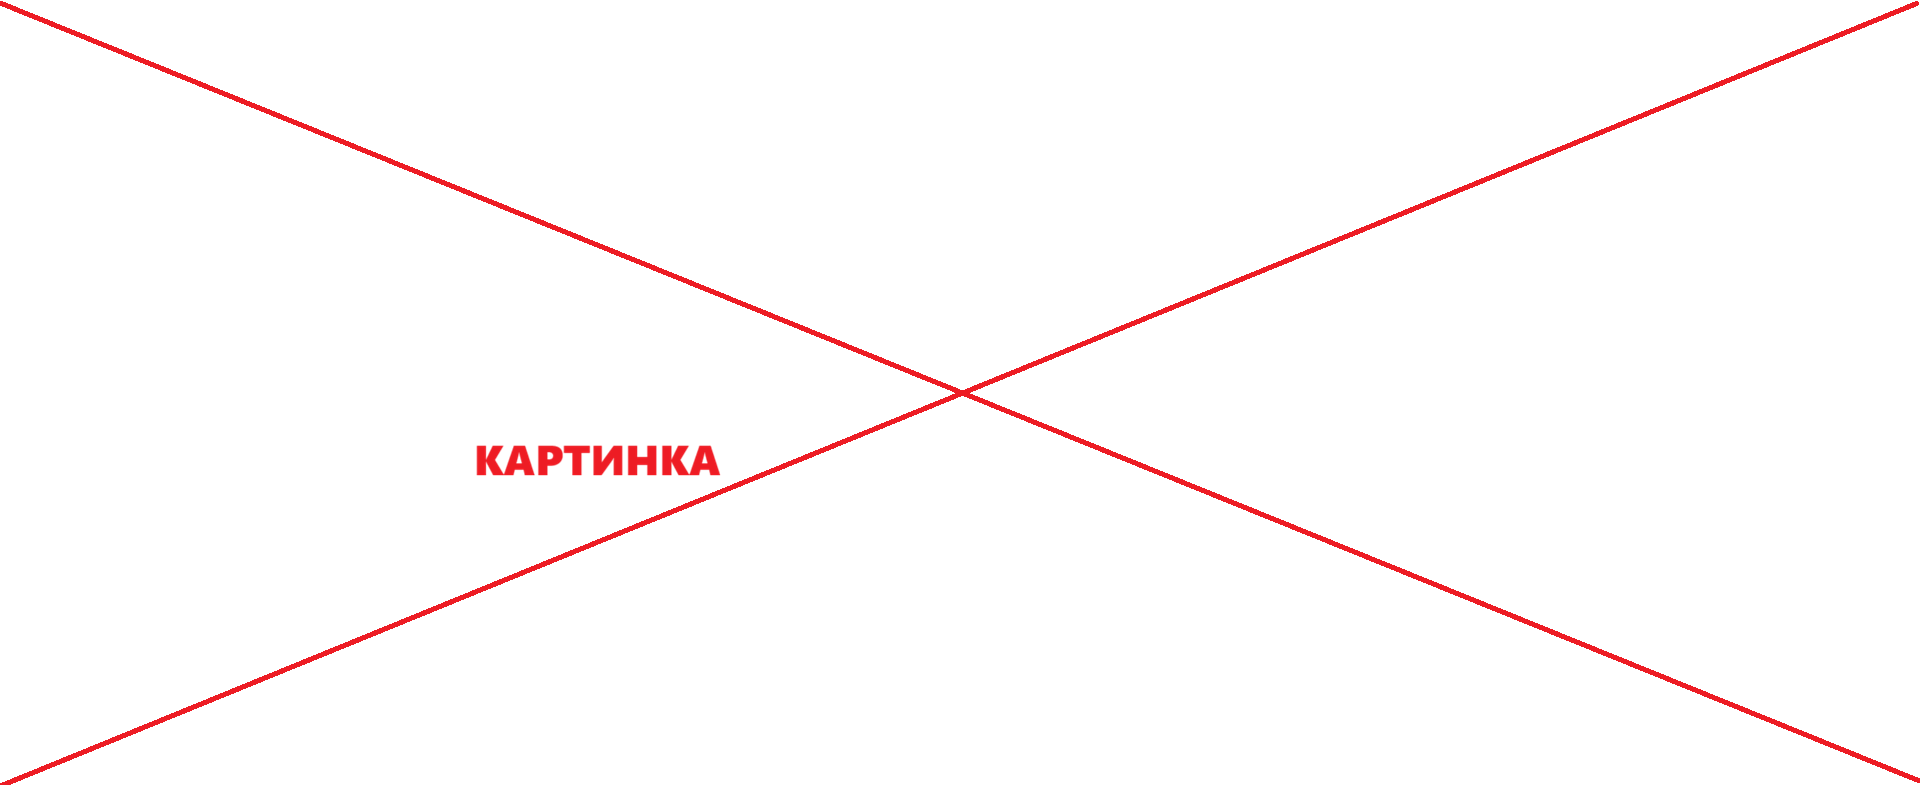
\includegraphics[scale=0.3]{template.png}
		\caption{\label{fig:template}Картинка многорамочного двигателя.}
	\end{figure}
	
	\subsection{Математическая модель электродвигателя}
	\quad
	Применим второй закон Кирхгофа к цепи ротора:
	\begin{equation}
		V_m(t)=\varepsilon_m+I_mR_m+L_m\dot{I}_m,
	\end{equation}
	где $\varepsilon_m=-\dfrac{d\Phi}{dt}$ - ЭДС индукции. Для рамки площадью $S=2aL$, вращающейся с угловой скоростью $\omega_m$, справедливо:
	\begin{equation}
		\dfrac{d\Phi}{dt}=\dfrac{d(SBcos\alpha)}{dt}=\dfrac{2aLB\cdot d[sin(-\phi)]}{dt}\approx -\dfrac{K_m\cdot d\phi}{dt}=-K_m\omega_m,
	\end{equation}
	где $\alpha$ - угол межлу нормалью к плоскости рамки и направлением поля, $\phi$ - угол между плоскости рамки и направлением поля.
	
	Пренебрегая индуктивностью $L_m$ (в силу малости), силой трения и считая момент инерции ротора с нагрузкой как $J_m$, уравнение динамики вращения:
	\begin{equation}
		J_m\dot{\omega}_m=K_mI_m.
	\end{equation}
	Подстановкой (7) в (5) (с учетом допущения малости $L_m$) исключим $I_m$:
	\begin{equation}
		V_m(t)=K_m\omega_m+\dfrac{J_mR_m}{K_m}\dot{\omega}_m.
	\end{equation}
	В изображениях Лапласа:
	\begin{equation}
		V_m(p)=\left(K_m+\dfrac{J_mR_m}{K_m}p\right)\omega_m(p),
	\end{equation}
	откуда коэффициент передачи электродвигателя
	\begin{equation}
		\boxed{K(p)=\dfrac{\omega_m(p)}{V_m(p)}=\dfrac{K_m}{R_mJ_mp+K^2_m}}.
	\end{equation}
	
	\section{Составление схемы управления электромотором}
	\subsection{Анализ динамического звена}
	\quad
	\textbf{Устойчивость.} Характеристическое уравнение $R_mJ_mp+K^2_m=0$ имеет единственный корень $p=-\dfrac{K_m^2}{R_mJ_m}<0$. Звено \textbf{асимптотически устойчиво} (далее - устойчиво).
	
	\textbf{Точность.} Подадим на вход звена $K(p)$ функцию Хевисайда $\mathcal{L}[\sigma(t)]=\dfrac{1}{p}$: 
	\begin{equation*}
		K(p)\cdot\dfrac{1}{p}=\dfrac{K_m}{p(R_mJ_mp+K_m^2)}=\dfrac{A}{p}+\dfrac{B}{p+a},
	\end{equation*}
	где $a=K^2_m/(R_mJ_m), A=1/K_m, B=-1/K_m$.
	Переходная функция:
	\begin{equation}
		H(t)=\mathcal{L}^{-1}\left[\frac{K(p)}{p}\right]=\frac{1}{K_m}(1-e^{-at}).
	\end{equation}
	
	\begin{figure}[H]
		\centering
		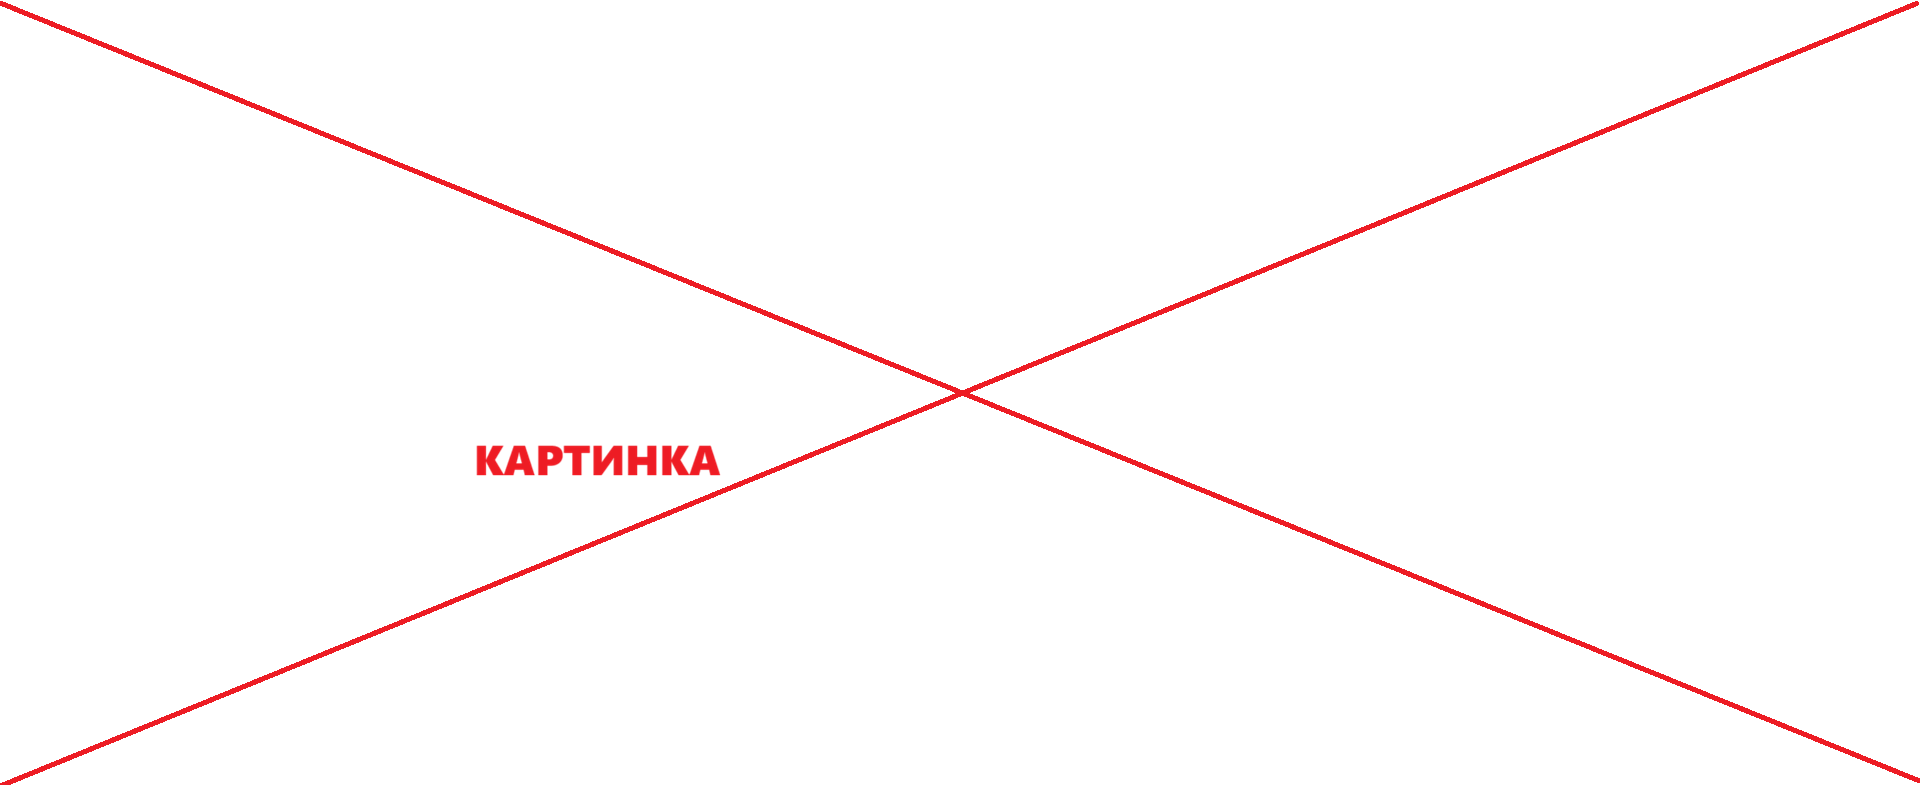
\includegraphics[scale=0.3]{template.png}
		\caption{\label{fig:template}График переходной функции}
	\end{figure}
	
	Звено \textbf{обладает точностью} (в смысле реакции на управление) с асимптотическим выходом на $\omega_m(\infty)=1/K_m$. Следовательно, управление скоростью звеном $K(p)$ при единичной помехе невозможно - рабочий режим определяется только параметрами двигателя $K_m$.
	
	\subsection{Управление с усилительным звеном (П-регулятор)}
	\quad
	Подключим последовательно усилительное звено с коэффициентом $K_p$ и замкнем систему отрицательной обратной связью по скорости (рис. 5). На вход полученного устройства подается желаемая угловая скорость $\omega_m^*(t)$. Ошибка $\varepsilon(t)=\omega_m^*(t)-\omega_m(t)$ подаётся на вход усилителя.
	
	\begin{figure}[H]
		\centering
		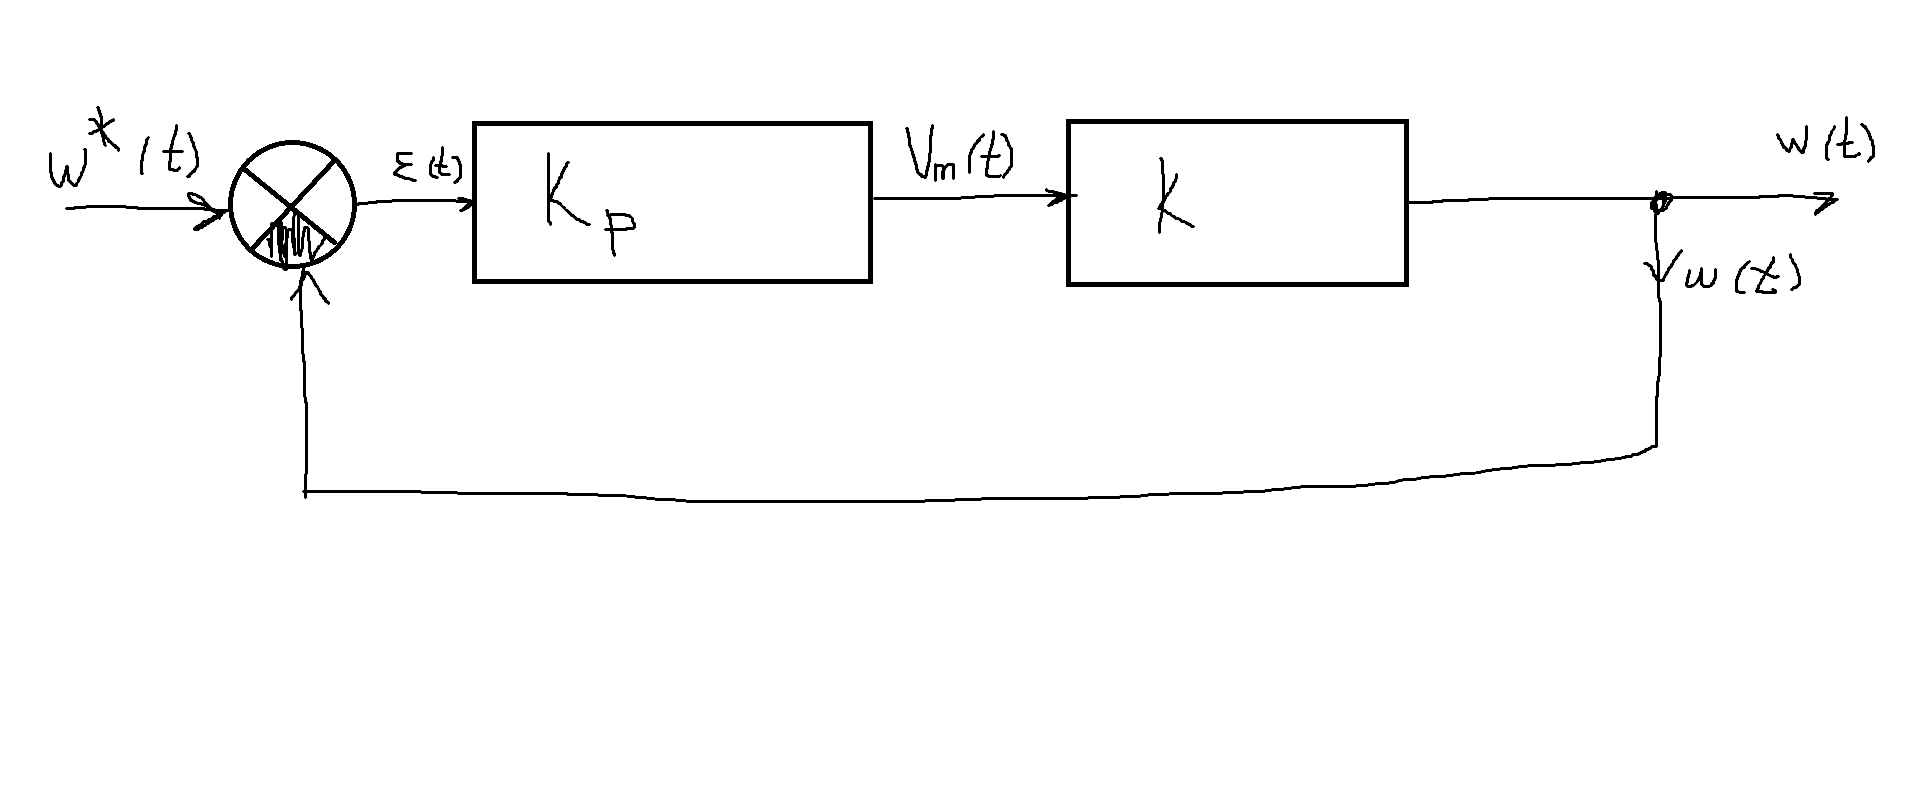
\includegraphics[scale=0.3]{amplifier_direct.png}
		\caption{\label{fig:amplifier_direct}Прямая диграмма звеньев с усилительным звеном. Перерисовать}
	\end{figure}
	
	Передаточная функция замкнутой системы:
	\begin{equation}
		K_{eq}(p)=\dfrac{\omega_m}{\omega^*_m}=\dfrac{K_mK_p}{R_mJ_mp+K_m^2+K_mK_p}.
	\end{equation}
	
	\textbf{Устойчивость.} Единственный корень знаменателя $p=-\dfrac{K_m^2+K_mK_p}{R_mJ_m} < 0$. Звено \textbf{устойчиво}.
	
	\textbf{Точность.} Подстановка $p=0$ (производная функции Хевисайда в изображениях) показывает, что звено \textbf{обладает точностью} (в смысле реакции на управление).
	Подадим на вход звена $K(p)$ функцию Хевисайда $\mathcal{L}[\sigma(t)]=\dfrac{1}{p}$: 
	\begin{equation*}
		K_{eq}(p)\cdot\dfrac{1}{p}=\dfrac{K_mK_p}{p(R_mJ_mp+K_m^2+K_mK_p)}=\dfrac{A}{p}+\dfrac{B}{p+\beta},
	\end{equation*}
	где $\beta=(K^2_m+K_mK_p)/(R_mJ_m), A=K_p/(K_m+K_p), B=-K_p/(K_m+K_p)$.
	
	Переходная функция:
	\begin{equation}
		H(t)=\mathcal{L}^{-1}\left[\frac{K_{eq}(p)}{p}\right]=\frac{K_p}{K_m+K_p}(1-e^{-\beta t}).
	\end{equation}
	
	\begin{figure}[H]
		\centering
		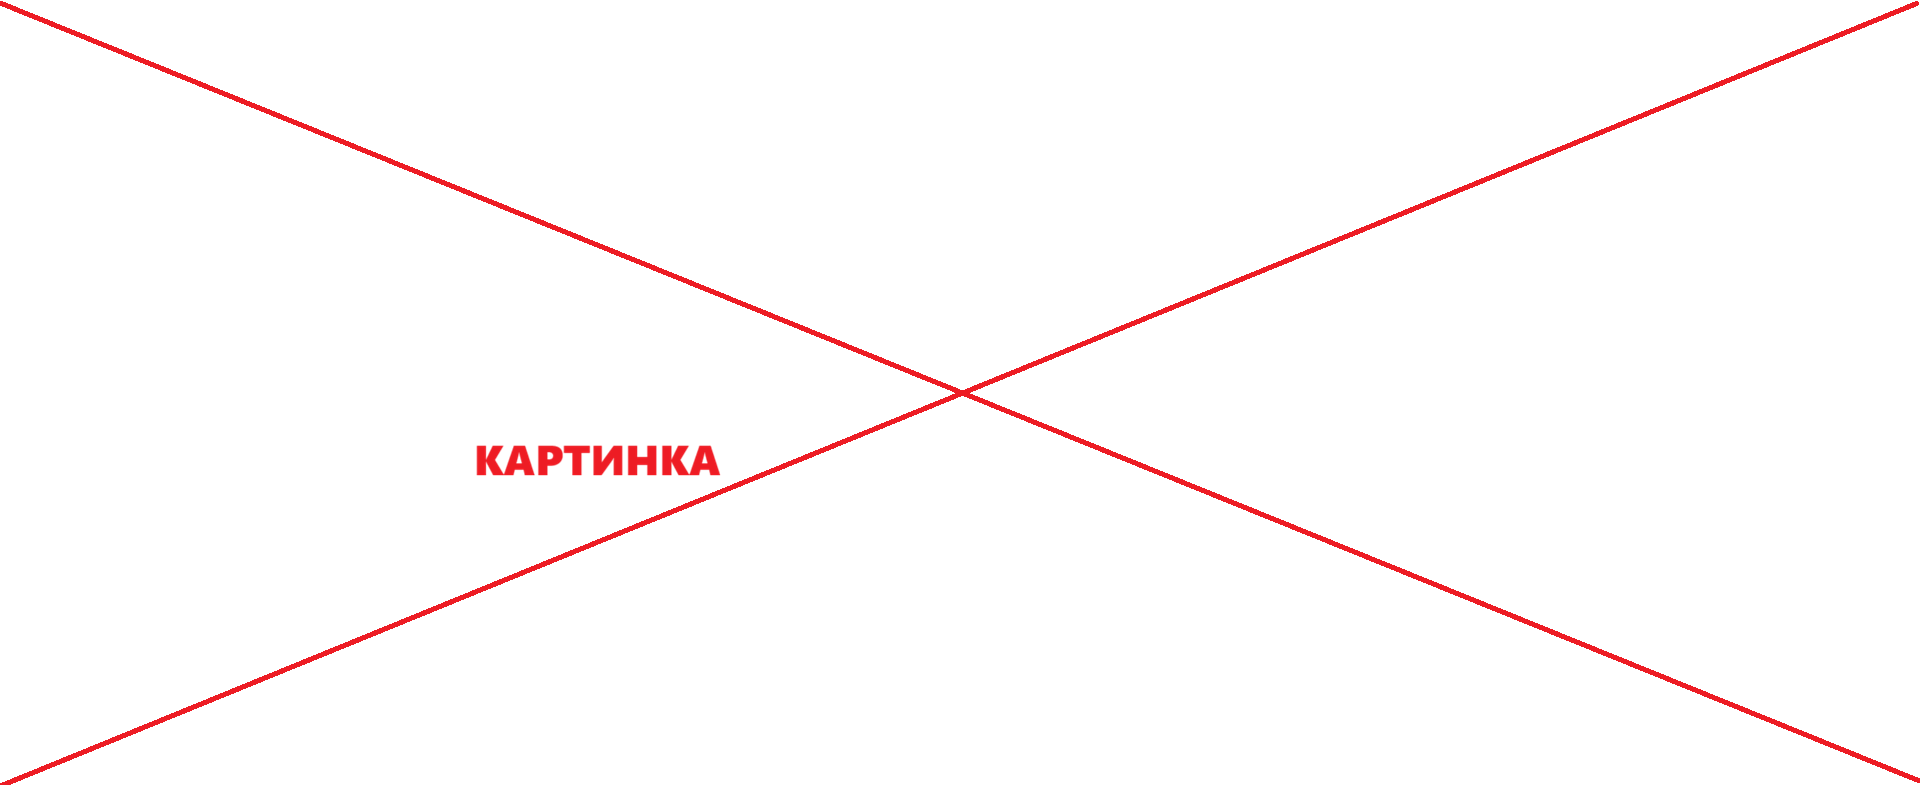
\includegraphics[scale=0.3]{template.png}
		\caption{\label{fig:template}График переходной функции}
	\end{figure}
	
	Система \textbf{асимптотически} выходит на $\omega_m(\infty)=K_p/(K_m+K_p)$ \textbf{без перерегулирования}, что позволяет достичь любой скорости вращения (при единичном полезном сигнале) в промежутке $(0;1)$ за счет изменения параметра П-регулятора $K_p\in(0;+\infty)$.
	
	\textbf{Время выхода в рабочий режим.} Считая рабочим режимом константу $\omega_m(\infty)=K_p/(K_m+K_p)$, найдем время входа $t^*$ в коридор $|\omega_m(\infty)-\omega_m(t)|\leq\delta$.
	\begin{equation*}
		|\omega_m(\infty)-\omega_m(t)| = \frac{K_p}{K_m+K_p}e^{-\beta t}\leq\delta\to t^*=\dfrac{1}{\beta}ln\left(\dfrac{K_p}{(K_m+K_p)\delta}\right)
	\end{equation*}
	\begin{equation}
		\boxed{ t^*=\dfrac{R_mJ_m}{K^2_m+K_mK_p}ln\left(\dfrac{K_p}{(K_m+K_p)\delta}\right)}.
	\end{equation}
	
	\textbf{Анализ ошибки.} Для оценки ошибки развернем схему, выделив коэффициент передачи по ошибке (рис. 7):
	
	\begin{equation}
		K_{\varepsilon\omega^*_m}(p)=\dfrac{\omega^*_m-\omega_m}{\omega^*_m}=\dfrac{R_mJ_mp+K_m^2}{R_mJ_mp+K_m^2+K_mK_p}.
	\end{equation}
	
	\begin{figure}[H]
		\centering
		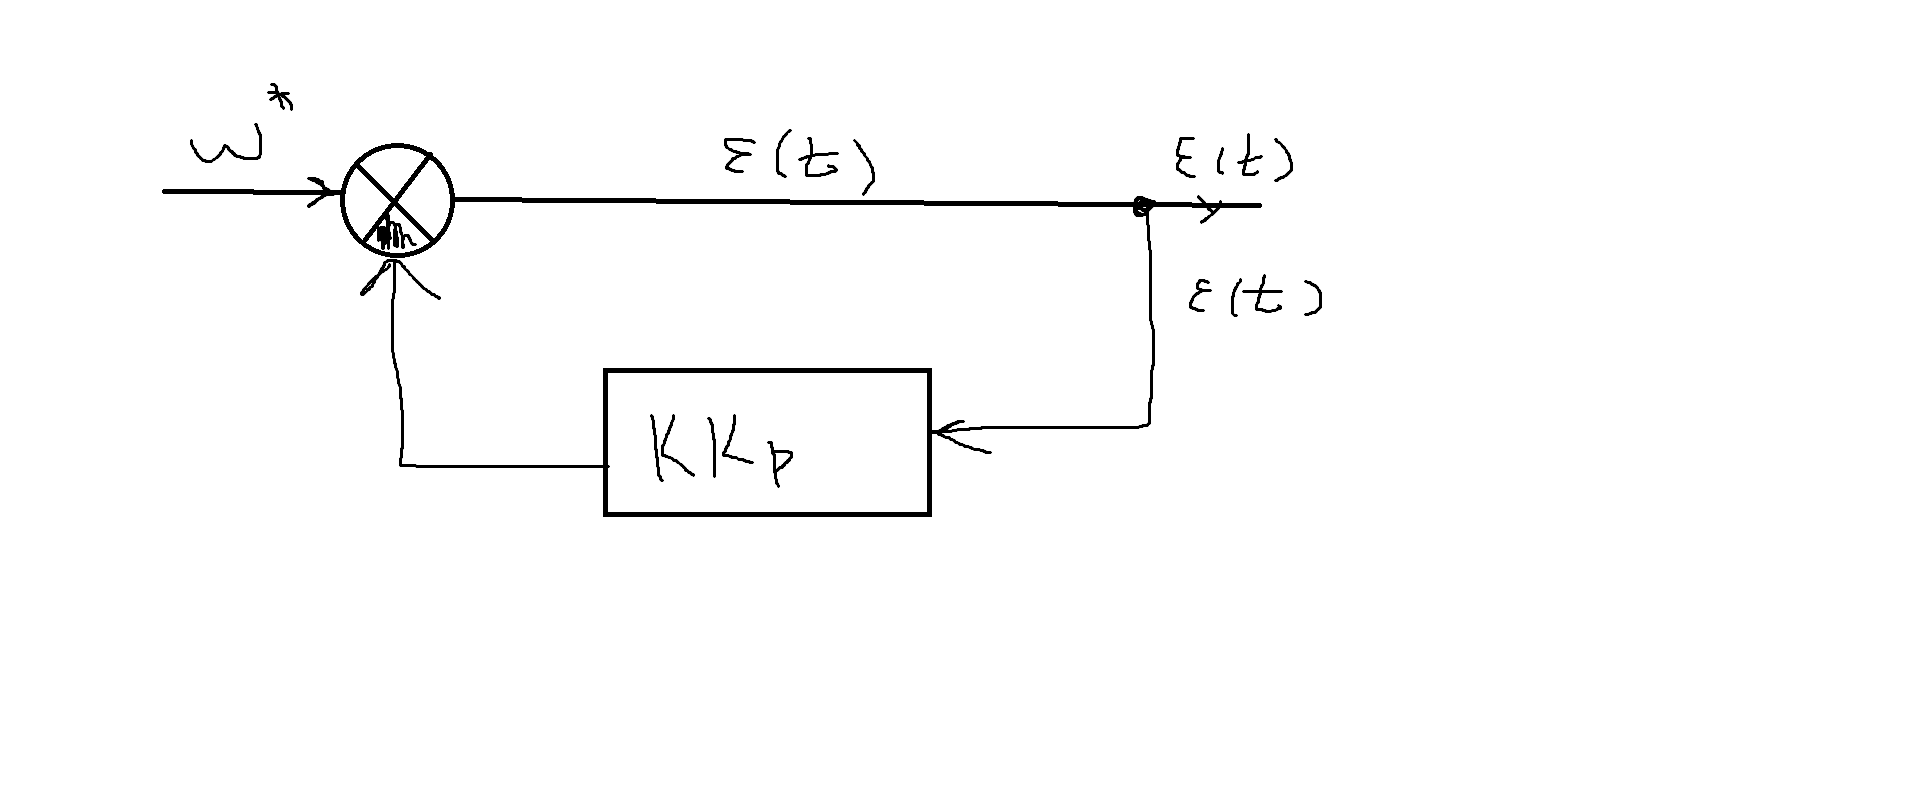
\includegraphics[scale=0.3]{amplifier_reverse.png}
		\caption{\label{fig:amplifier_reverse}Обращённая диграмма звеньев с усилительным звеном. Перерисовать}
	\end{figure}
	
	В силу $K_{\varepsilon\omega^*_m}(0)=\dfrac{K_m}{K_m+K_p}$ звено $K_{eq}(p)$ \textbf{обладает неустранимой ошибкой} выхода в рабочий режим, величина которой стремится к $\varepsilon(\infty)=\dfrac{K_m}{K_m+K_p}$. Зависимость от $K_p$ позволяет контролировать ошибку, благодаря чему имеет место задача подбора параметра звена для выхода в некоторый коридор желаемого режима (например, с заданной абсолютной погрешностью не более $\delta^*$).
	Получаем условие:
	\begin{equation}
		\varepsilon(\infty)=\dfrac{K_m}{K_m+K_p}\leq\delta^*\to \boxed{ K_p\geq\dfrac{1-\delta^*}{\delta^*}K_m}.
	\end{equation}
	
	Теоретически П-регулятор способен обеспечить сколь угодно малую конечную ошибку за счет увеличения $K_p$, однако на практике такое устройство будет иметь существенные ограничения. Поскольку $V_m(p)=K_p\varepsilon(p)$, а рабочее напряжение электродвигателя зачастую (из физических соображений) невелико, большие значения $K_p$ приводят к превышению допустимого напряжения во время переходного процесса (пока $\varepsilon$ недостаточно мало).
	
	\subsection{Управление с интегрирующим звеном (И-регулятор)}
	\quad
	Заменим усилительное звено интегрирующим с коэффициентом $K_i$ (рис. 8). 
	
	\begin{figure}[H]
		\centering
		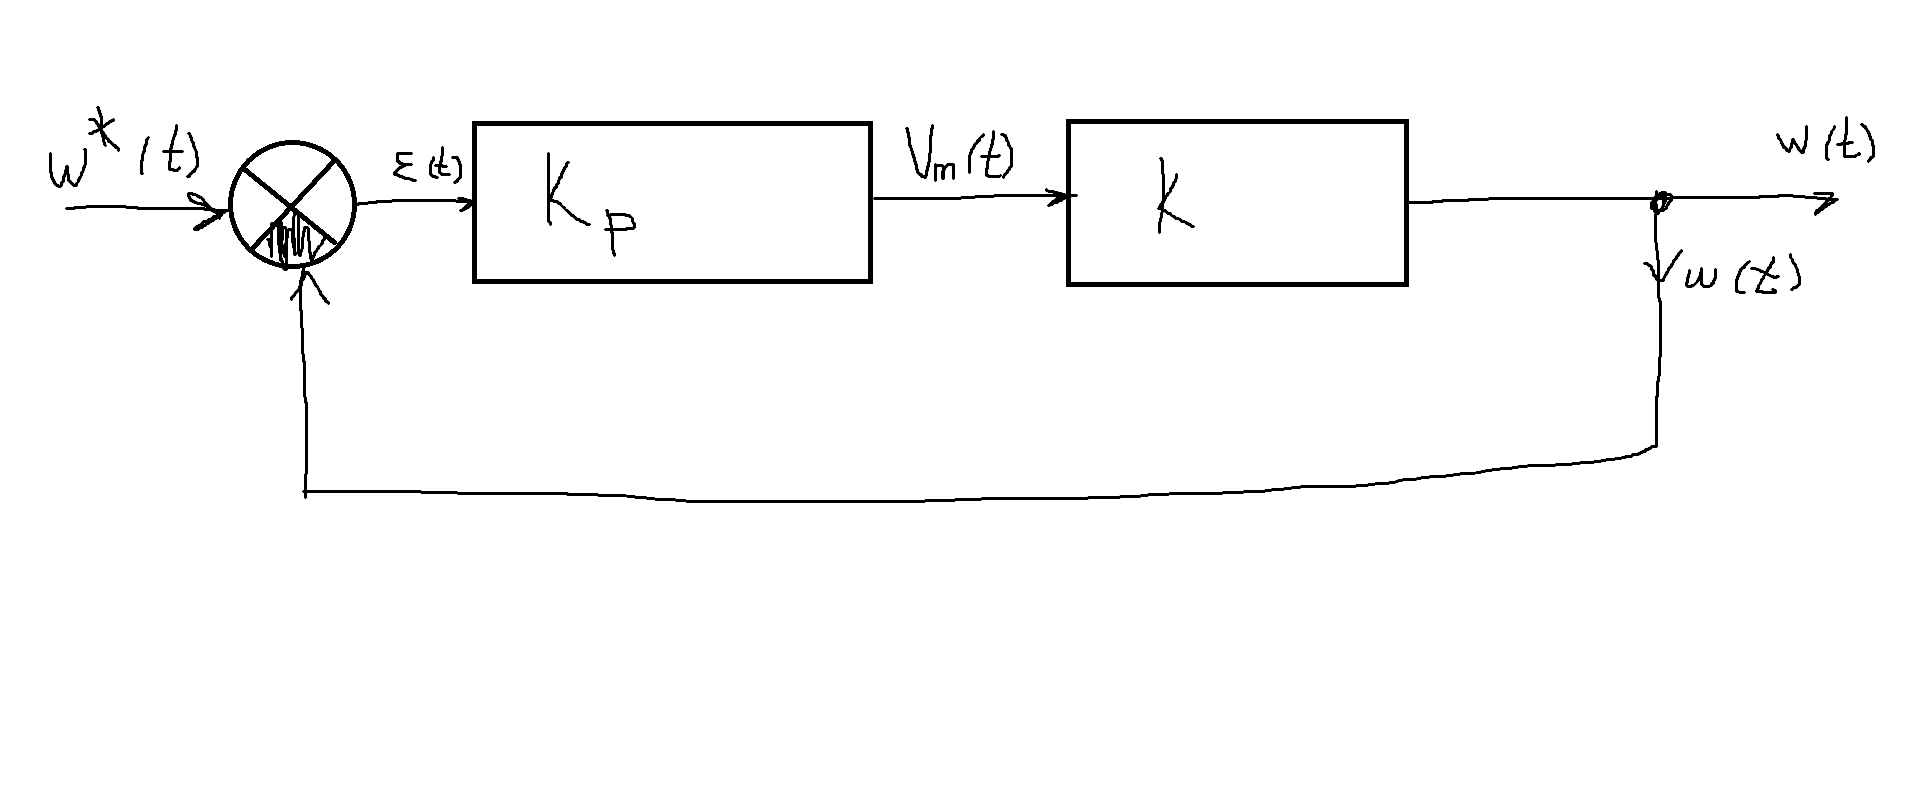
\includegraphics[scale=0.3]{amplifier_direct.png}
		\caption{\label{fig:integrator_direct}Прямая диграмма звеньев с интегрирующим звеном. Перерисовать}
	\end{figure}
	
	Коэффициент передачи замкнутой системы:
	\begin{equation}
		K_{eq}(p)=\dfrac{\omega_m}{\omega^*_m}=\dfrac{K_iK_m}{R_mJ_mp^2+K_m^2p+K_iK_m}.
	\end{equation}
	
	\textbf{Устойчивость.} Характеристический полином второго порядка $R_mJ_mp^2+K_m^2p+K_iK_m$ удовлетворяет необходимому и достаточному условию устойчивости при $K_i>0$. С учетом ограничения звено \textbf{устойчиво}.
	
	\begin{figure}[H]
		\centering
		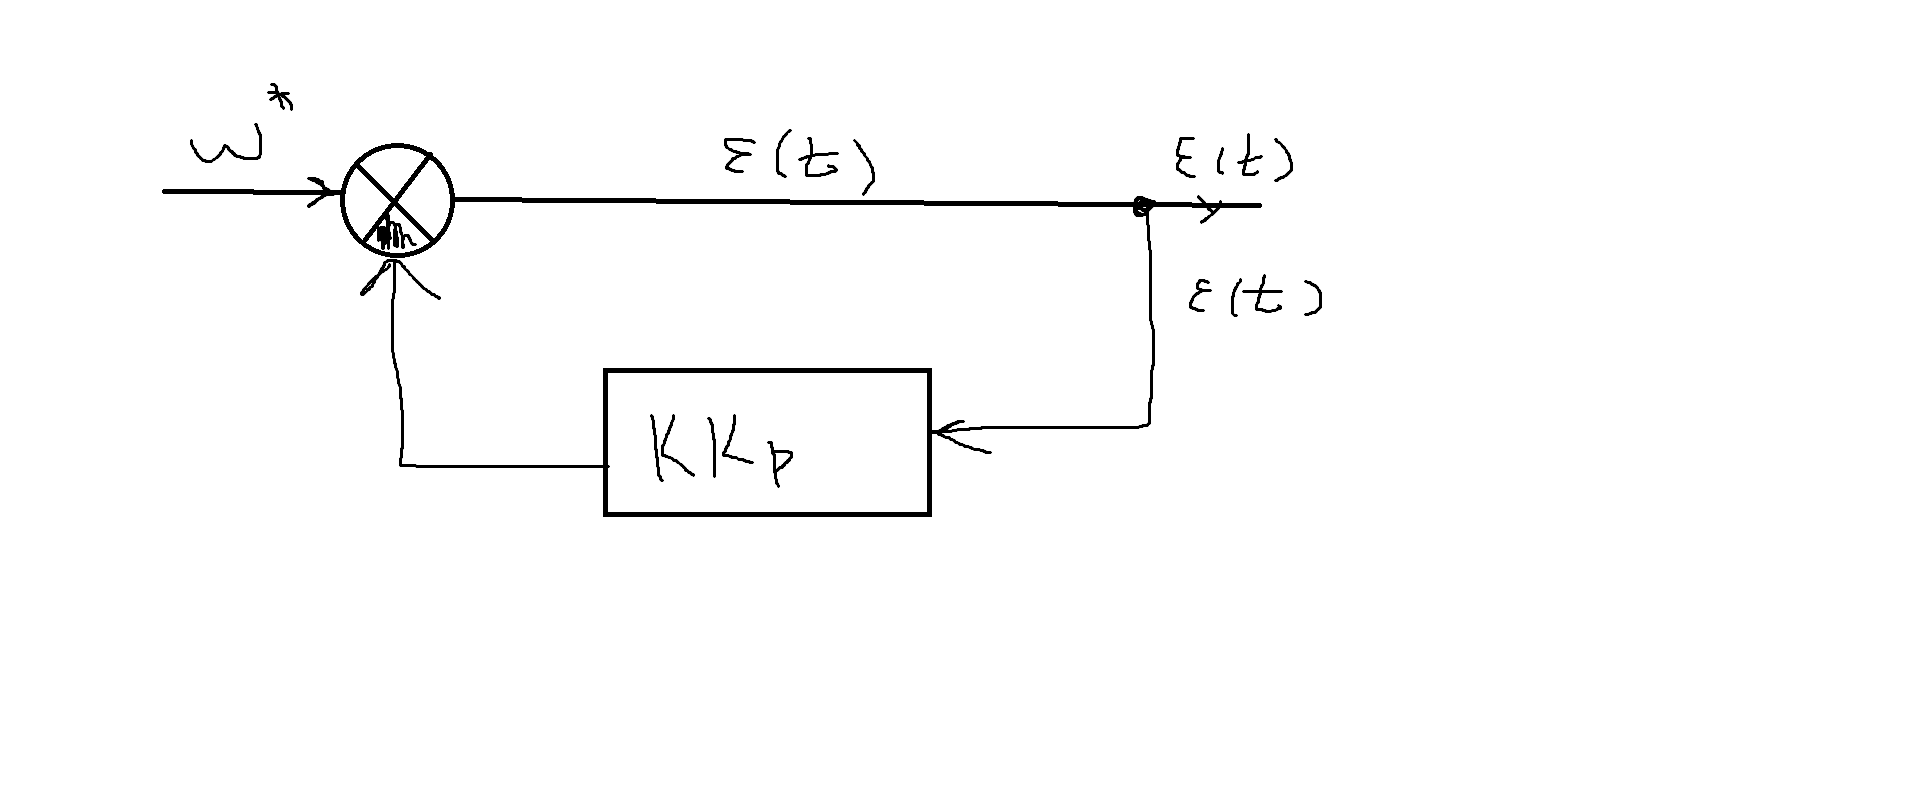
\includegraphics[scale=0.3]{amplifier_reverse.png}
		\caption{\label{fig:integrator_direct}Обратная диграмма звеньев с интегрирующим звеном. Перерисовать}
	\end{figure}
	
	Коэффициент передачи $K_{\epsilon\omega_m^*}(p)=\dfrac{p}{p+K_iK}\Rightarrow{}K{\epsilon\omega_m^*}(0)=0$, то есть реакция ошибки при подаче в качестве сигнала функции Хэвисайда - обратиться к 0, то есть исходный коэффициент передачи $K_{int}(p)$ обладает точностью.
	
	\textbf{Точность.} Подстановка $p=0$ показывает, что звено \textbf{обладает точностью} (в смысле реакции на управление).
	
	Переходная функция. Рассмотрим 3 вида переходной функции в зависимости от различной конфигурации корней характеристического уравнения: действительных различных, действительных кратных и комплексно-сопряженных.
	
	Вид переходной функции зависит от корней характеристического полинома:
	\begin{equation}
		p_{1,2}=\dfrac{-K_m^2\pm\sqrt{K^4_m-4R_mJ_mK_iK_m}}{2R_mJ_m}.
	\end{equation}
	
	\begin{itemize}
		\item \textit{Вещественные различные} корни $p_1<p_2<0$:
		\begin{equation}
			\boxed{ 0\ <\ K_i<\dfrac{K_m^3}{4R_mJ_m}} \label{eq19}			
		\end{equation}
		
		\begin{equation*}
			\dfrac{K_{eq}(p)}{p}=\dfrac{K_iK_m}{p(R_mJ_mp^2+K_m^2p+K_iK_m)}=\dfrac{1}{p}+\dfrac{B}{p-p_1}-\dfrac{C}{p-p_2},
		\end{equation*}
		где $B=\dfrac{K_iK_m}{R_mJ_mp_1(p_1-p_2)}$, $C=\dfrac{K_iK_m}{R_mJ_mp_2(p_1-p_2)}$ $\to C>B>0$.
		
		В оригиналах переходная функция запишется как
		\begin{equation}
			H(t)=1+Be^{p_1t}-Ce^{p_2t}.
		\end{equation}
		
	
	В моделировании далее будут использованы следующие подбираемые параметры модели:
\begin{itemize}
	\item $R_m = 3~\text{Ом}$
	\item $K_m = 0.02~\text{В/(рад/с)}$
	\item $J_{eq} = 2.00 \times 10^{-5}~\text{кг} \cdot \text{м}^2$
	\item $\text{Критическое значение}~ K_{i}= 0.033333$ вычисленное по формуле \ref{eq19}
	\item Желаемый режим - 5\% от $\omega^*$
\end{itemize}
	
	\begin{figure}[H]
		\centering
		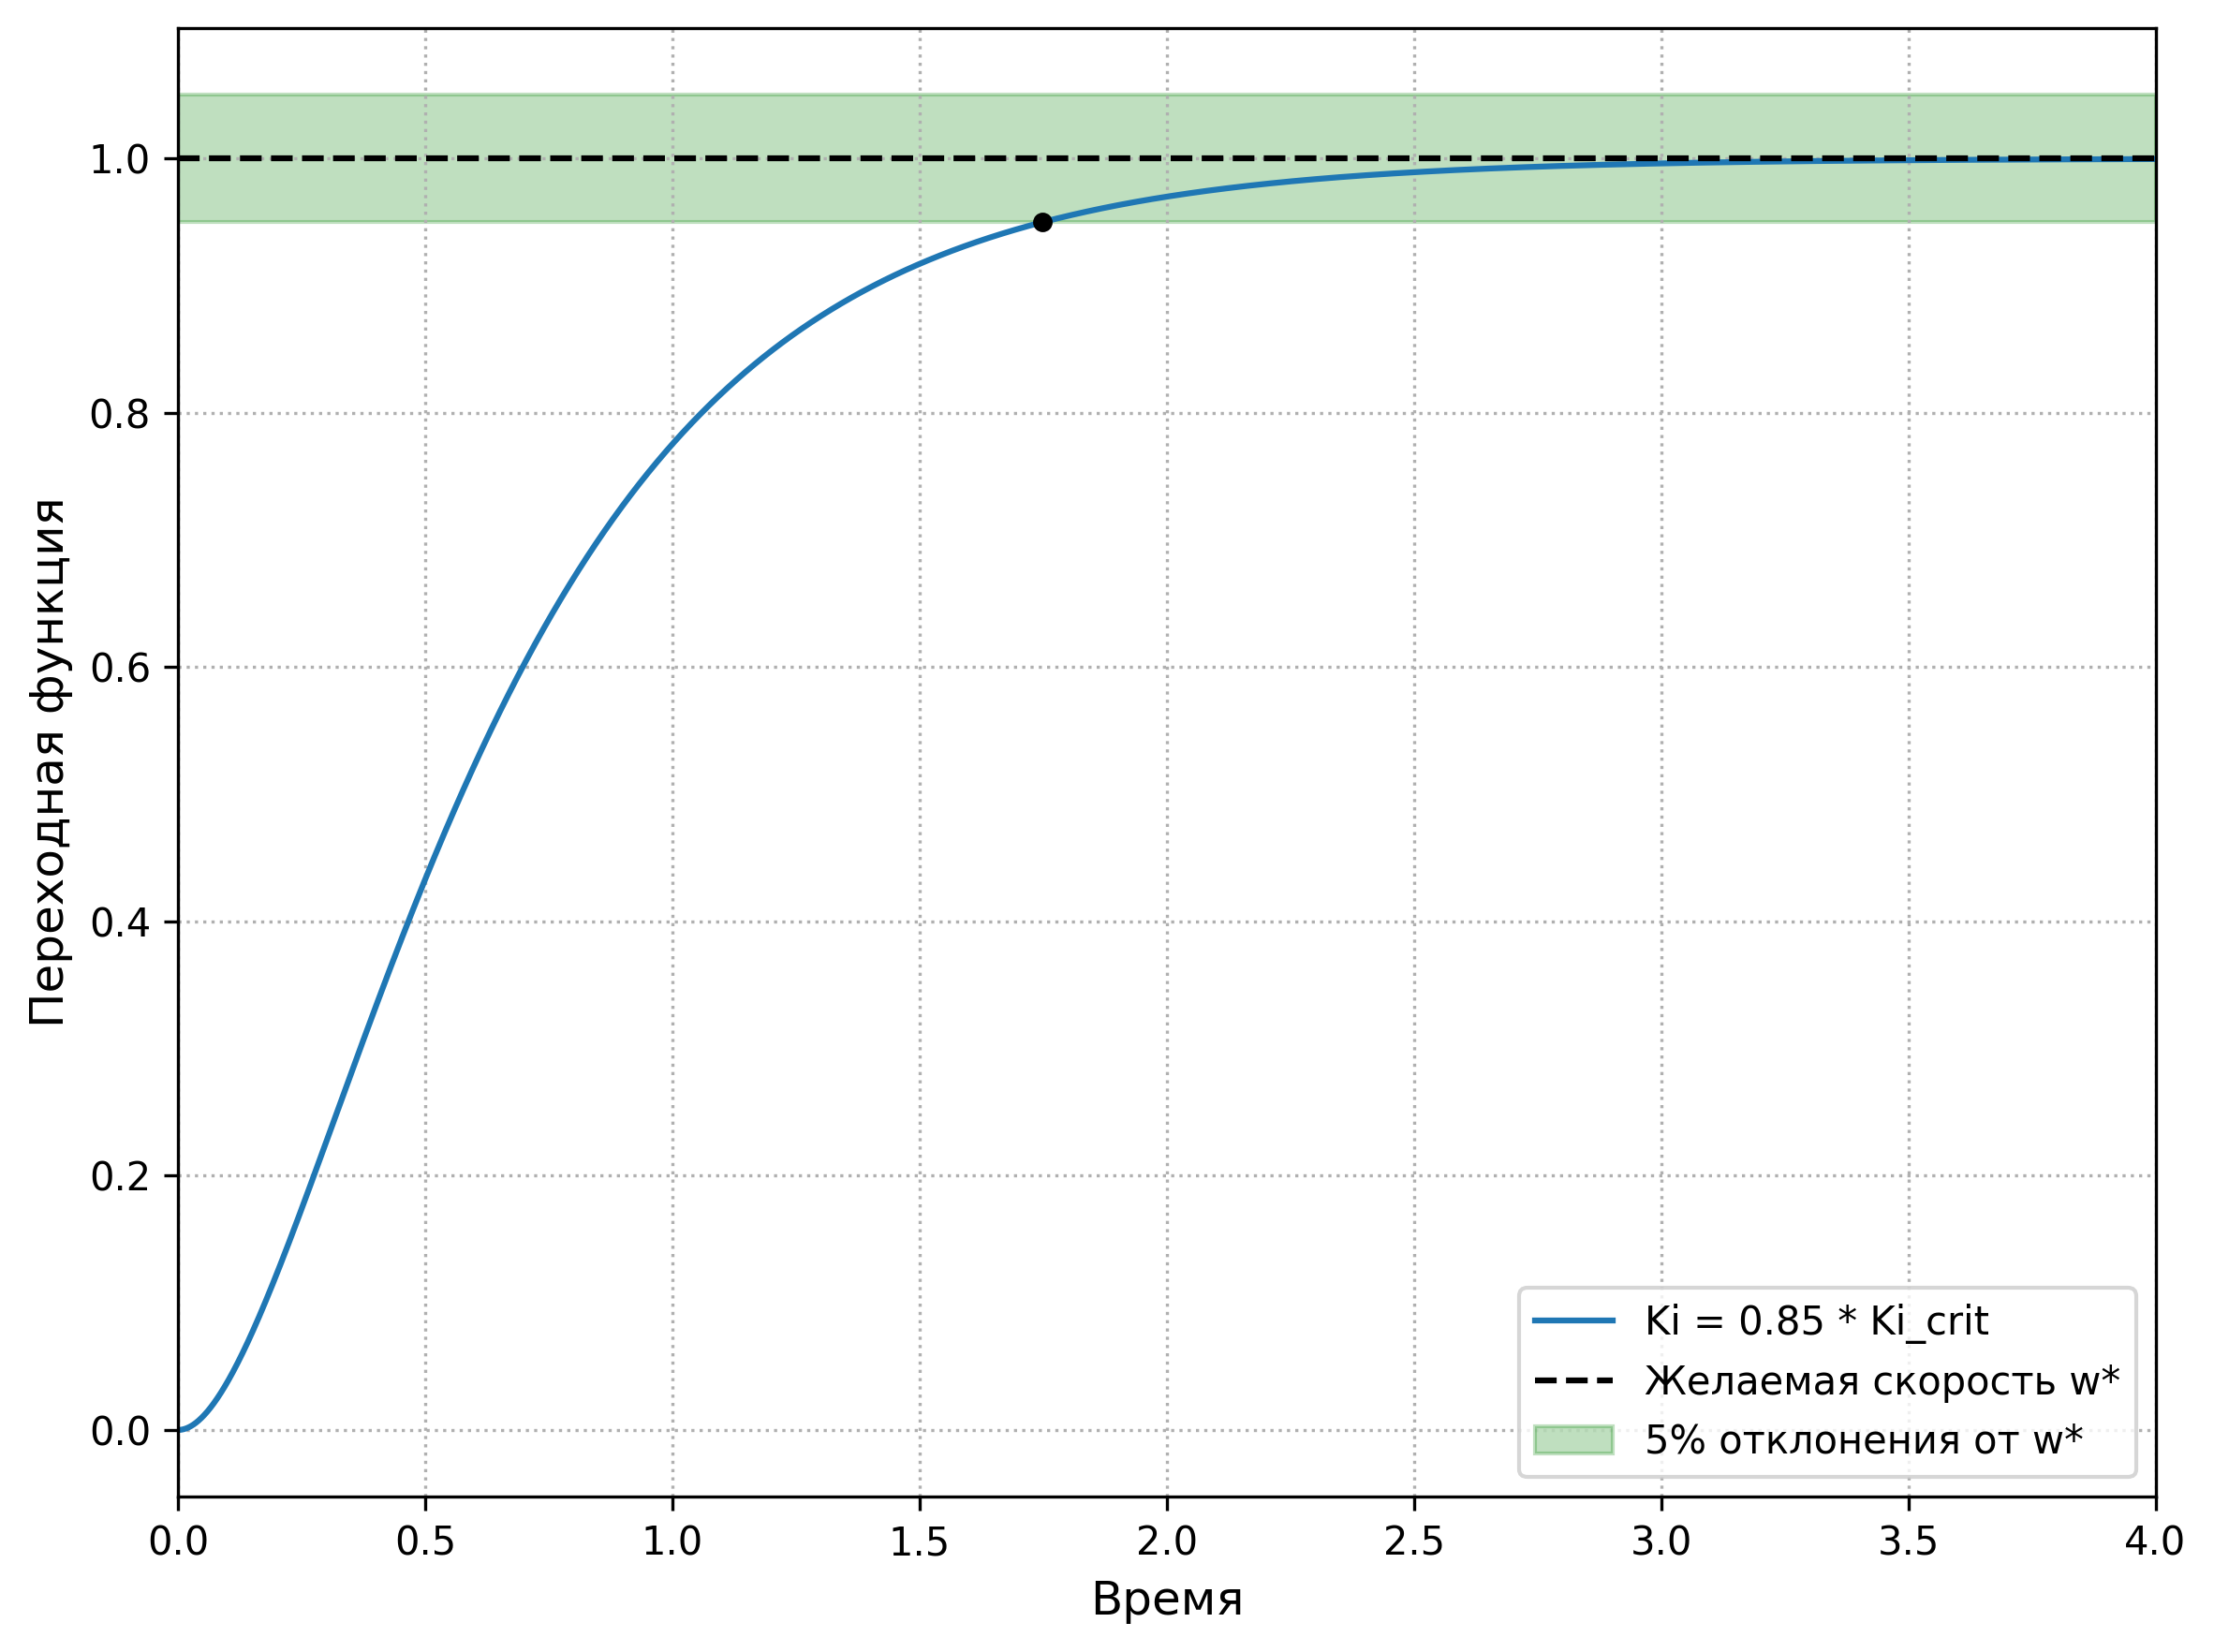
\includegraphics[scale=0.8]{graphic_aperiodic.png}
		\caption{\label{fig:graphic_aperiodic}График переходной функции при различных вещественных корнях}
	\end{figure}
	
	Обозначим данную траекторию номером 1 в таблице \ref{tab:table1}.
	
	При вещественных различных корнях происходит апериодический выход на константу без перерегулирования. Долгое время входа из-за наличия медленно затухающей экспоненты соответствующей ${p_2}$. Чем ближе K\_i к критическому значению, тем быстрее траектория входит в коридор и тем меньше ошибка.
	
		\item \textit{Кратный} корень $p_0=-\dfrac{K^2_m}{2R_mJ_m}$:
		\begin{equation}
			\boxed{ K_i=\dfrac{K_m^3}{4R_mJ_m}}
		\end{equation}
		
		\begin{equation*}
			\dfrac{K_iK_m}{p(R_mJ_mp^2+K_m^2p+K_iK_m)}=\dfrac{1}{p}-\dfrac{1}{p-p_0}-\dfrac{p_0}{(p-p_0)^2}.
		\end{equation*}
		
		Переходная функция:
		\begin{equation}
			H(t)=1-e^{p_0t}+p_0te^{p_0t}.
		\end{equation}
		
		\begin{figure}[H]
			\centering
			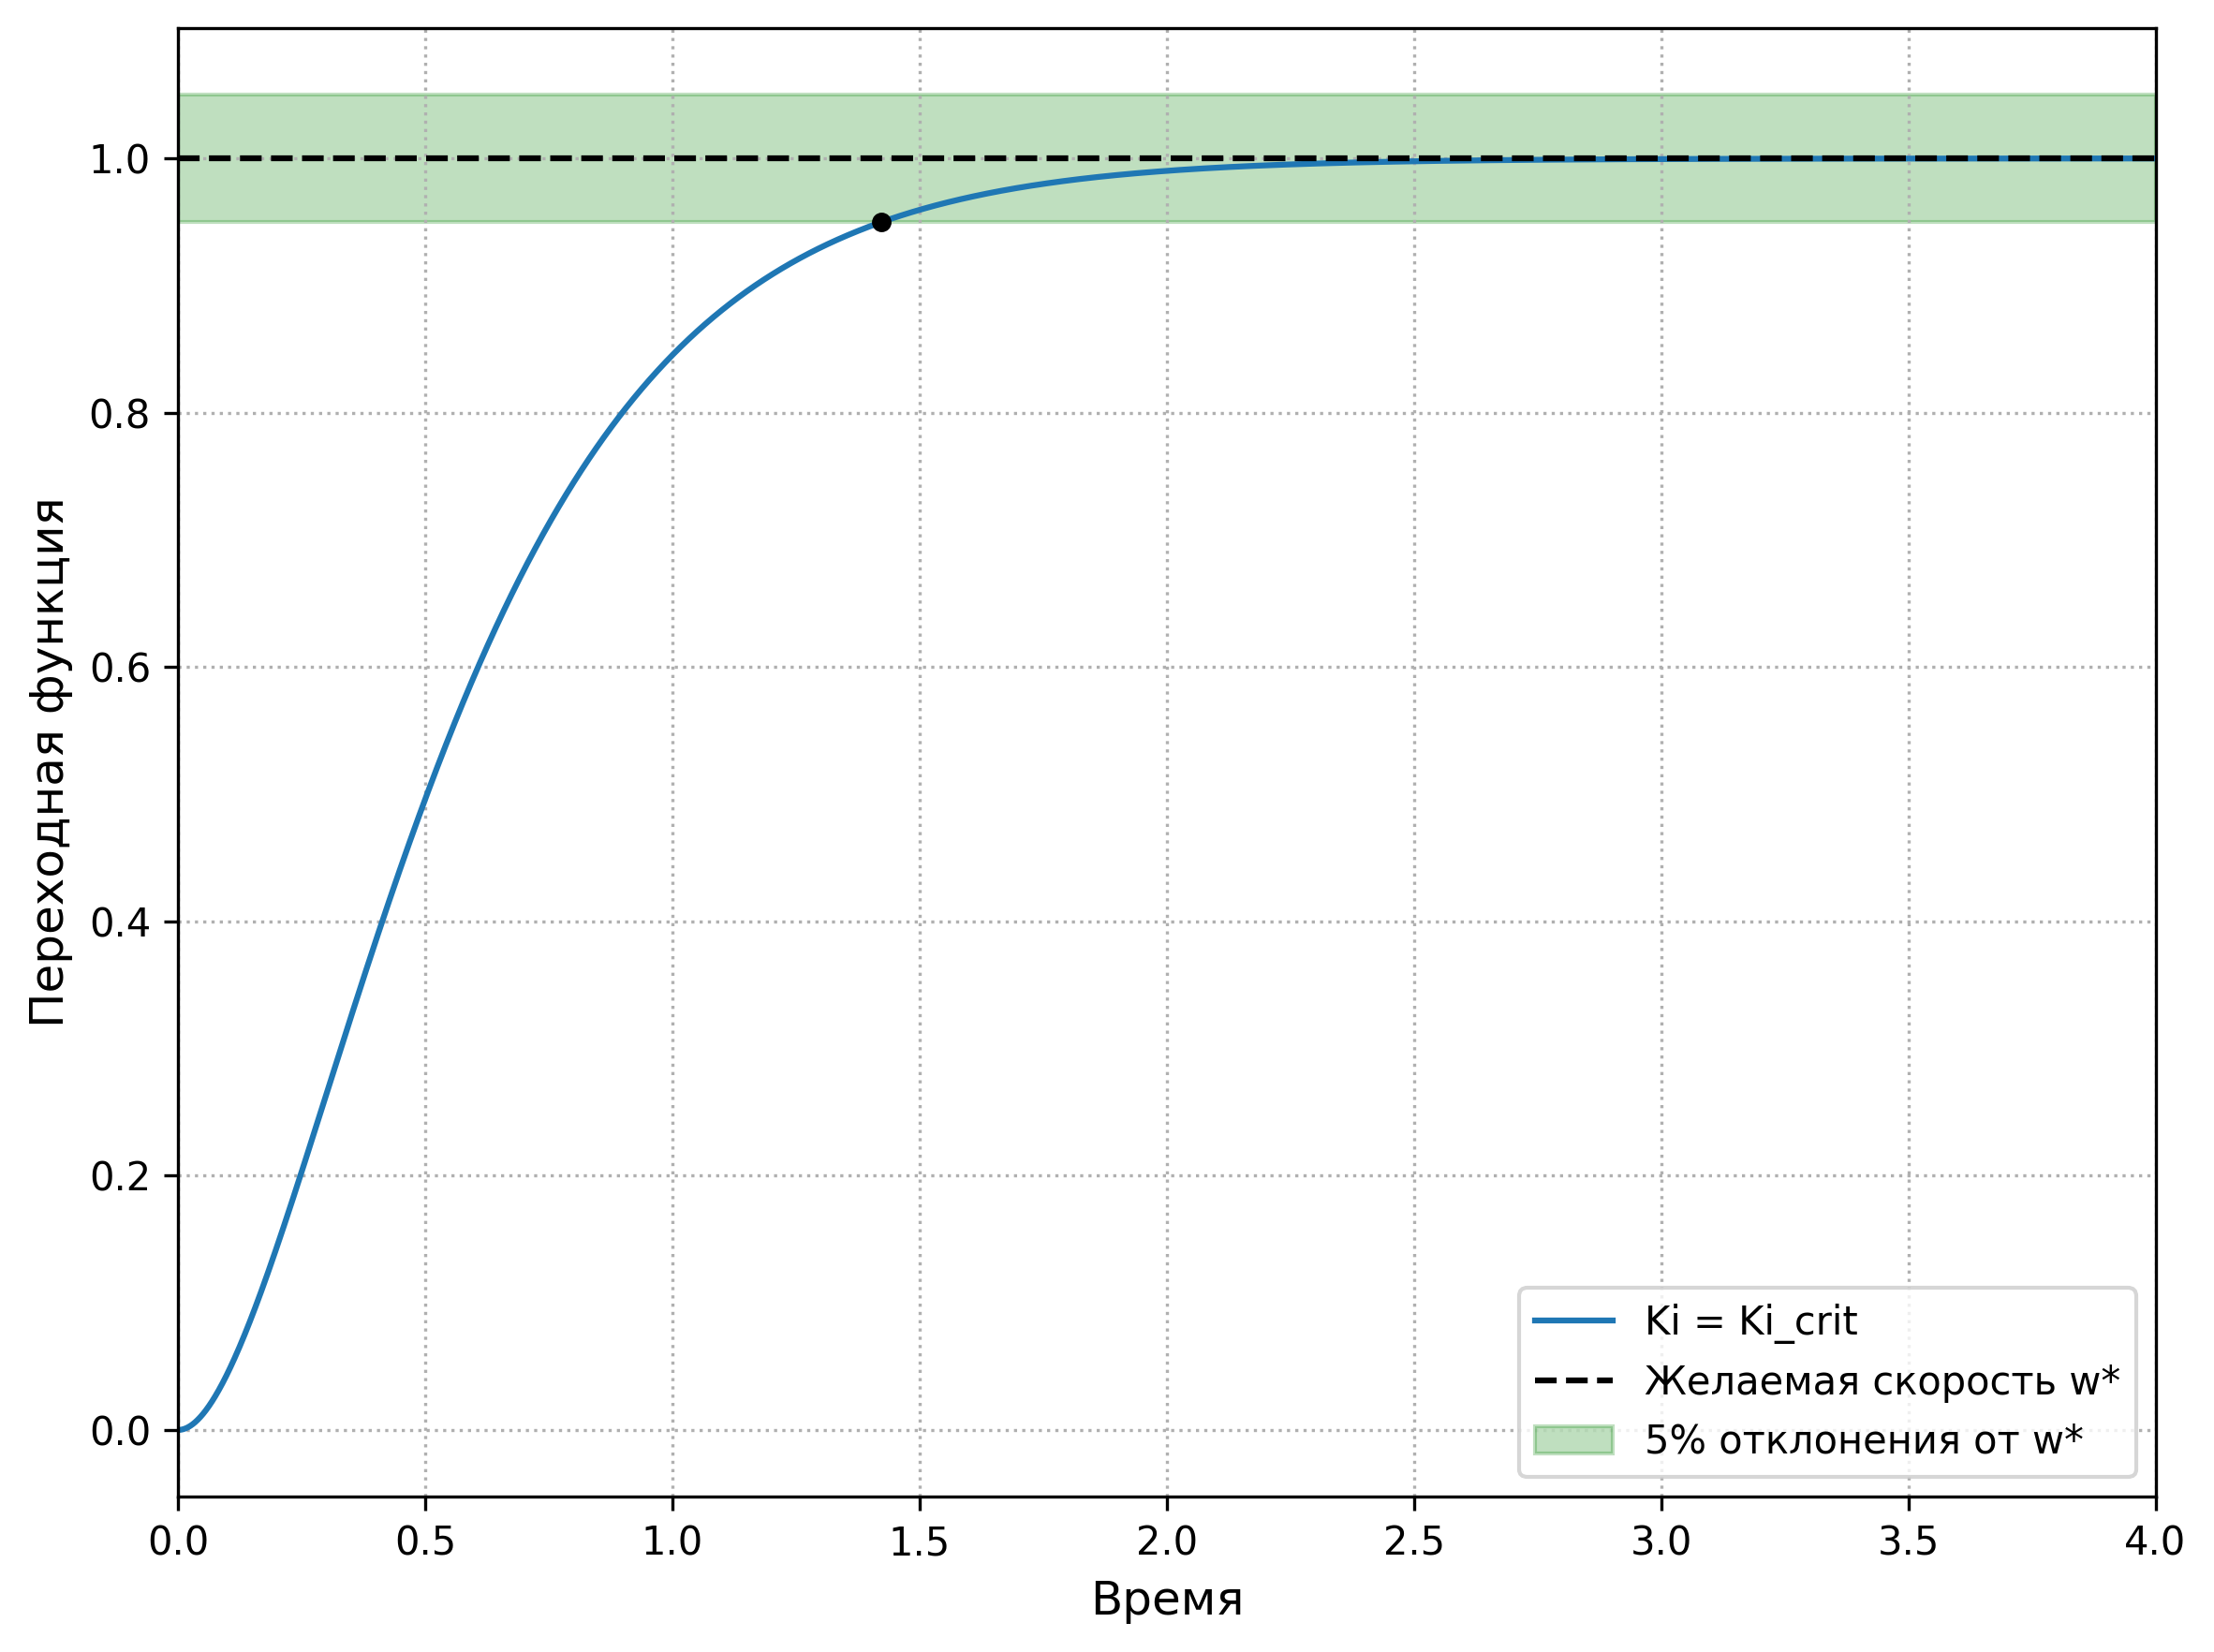
\includegraphics[scale=0.8]{graphic_critical.png}
			\caption{\label{fig:graphic_critical}График переходной функции при кратном вещественном корне}
		\end{figure}
		
		Обозначим данную траекторию номером 2 в таблице \ref{tab:table1}.
	
		При вещественном кратном корне происходит апериодический выход на константу без перерегулирования. Данный $K_i$ обеспечивает минимальное время выхода в рабочий режим без перерегулирования.
		
		\item \textit{Комплексно-сопряженные} корни $p_{1,2}=-\alpha\pm i\beta$,
		
		где $\alpha=\dfrac{K^2_m}{2R_mJ_m}$, $\beta=\dfrac{\sqrt{4R_mJ_mK_iK_m-K^4_m}}{2R_mJ_m}$:
		\begin{equation}
			\boxed{ K_i>\dfrac{K_m^3}{4R_mJ_m}}
		\end{equation}
		
		Справедливы тождества:
		\begin{equation*}
			\dfrac{K_{eq}(p)}{p}=\dfrac{1}{p}\cdot\dfrac{\alpha^2+\beta^2}{(p+\alpha)^2+\beta^2}=\dfrac{1}{p}-\dfrac{p+2\alpha}{(p+\alpha)^2+\beta^2}.
		\end{equation*}
		
		Обратное преобразование Лапласа дает переходную функцию:
		\begin{equation}
			H(t)=1-e^{-\alpha t}\left(\cos(\beta t)+\dfrac{\alpha}{\beta}\sin(\beta t)\right).
			\label{eq24}
		\end{equation}
		
		\begin{figure}[H]
			\centering
			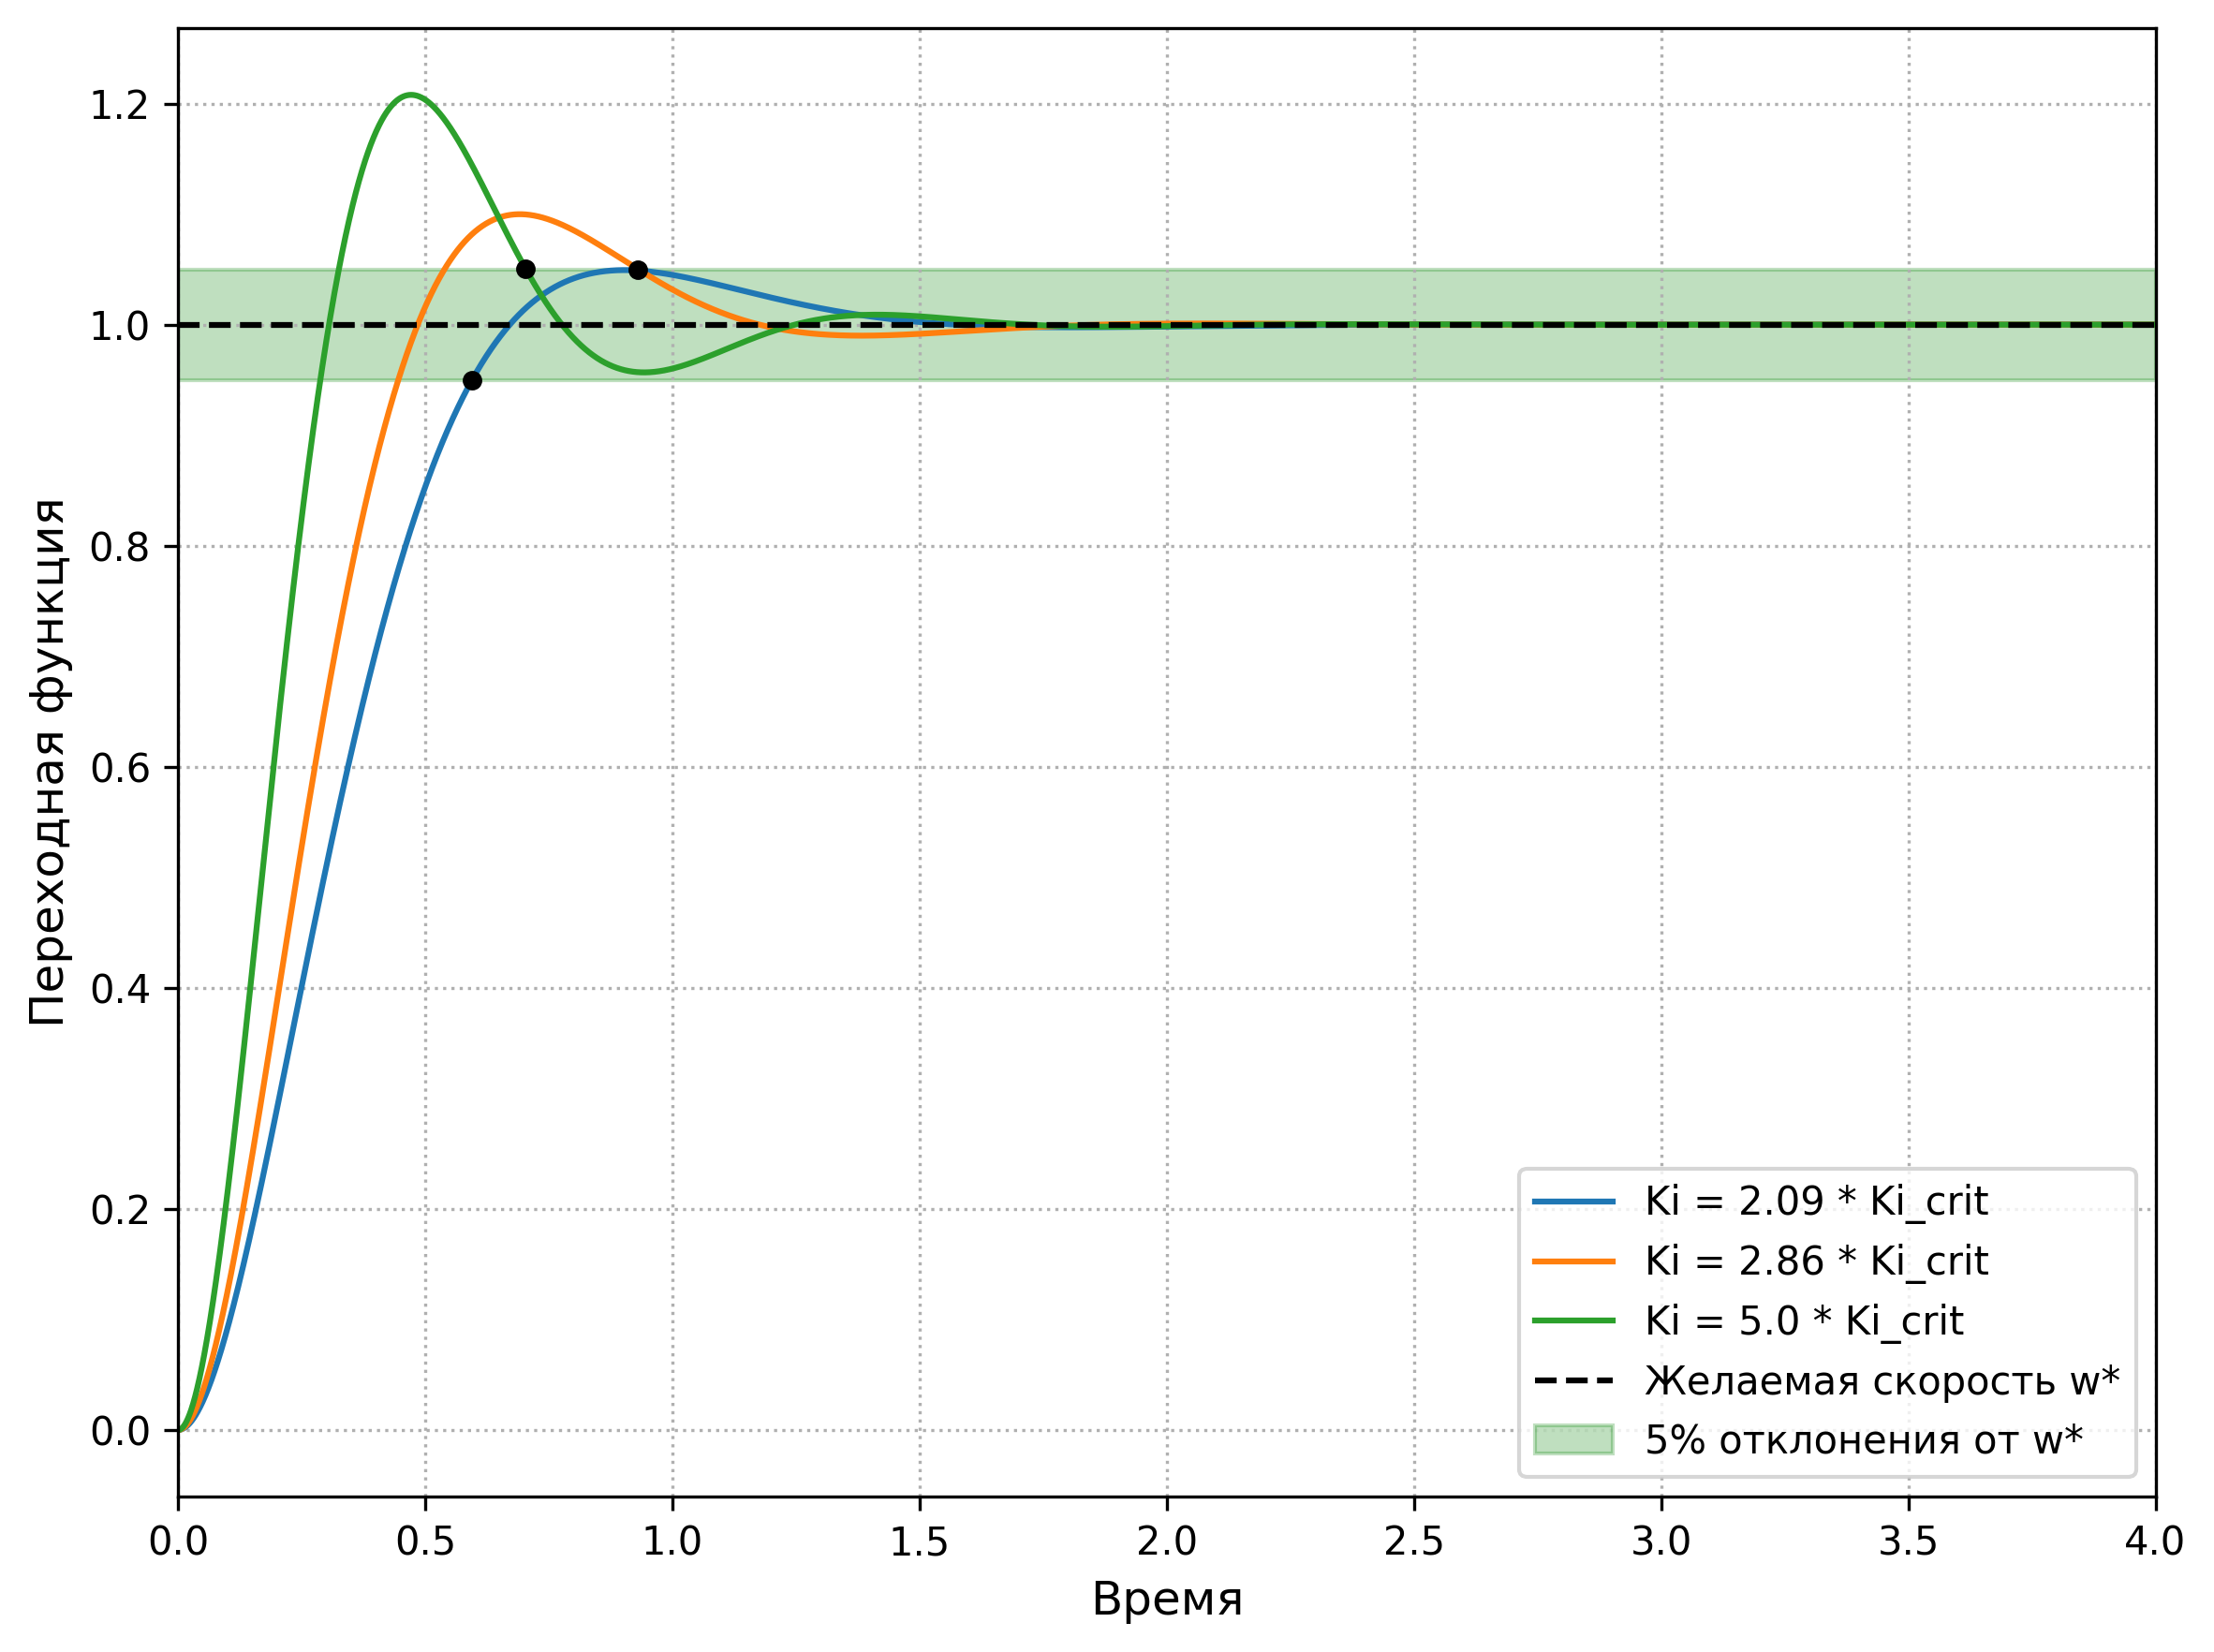
\includegraphics[scale=0.8]{graphic_oscillatory.png}
			\caption{\label{fig:graphic_oscillatory}График переходной функции при комплексных корнях}
		\end{figure}

		Обозначим синюю, жёлтую и зелёную траекторию на данном рисунке номерами 3, 4 и 5 соответственно в таблице \ref{tab:table1}.

		При комплексно-сопряжённых корнях происходит колебательный выход на константу с перерегулированием. Данный $K_i$ обеспечивает минимальное время выхода в рабочий режим, но нужно контролировать значение перерегулирования (иначе будет перегруз устройства).
		
		Часто в реальных задачах максимальных выброс переходной функции может быть ограничен, поэтому найдём его значение, для этого продифференцируем \ref{eq24}:
		
		\begin{equation}
			H'(t)=e^{-\alpha t} \frac{\alpha^2 + \beta^2}{\beta}sin(\beta t).
		\end{equation}
		
		Получаем время максимально выброса: $t_{max} = \frac{\pi}{\beta}$
		
		Подставляя это время, получаем значение максимального выброса: 
		\begin{equation}
			H_{max} = H(t_{max}) = 1 + e^{\frac{-\alpha\pi}{\beta}}
		\end{equation}
		
		Наложим ограничение на $H_{max}$, пусть максимальный выброс не превышает 10\%:
		
		\begin{equation}
			H_{max} = 1 + e^{\frac{-\alpha\pi}{\beta}} \leq 1.1
		\end{equation}
		
		Подставляя значения $\alpha$ и $\beta$ и выражая $K_i$, получаем следующее неравенство:
		
		\begin{equation}
			K_i \le \frac{K_m^3}{4 R_m J_m} \left( 1 + \frac{\pi^2}{(\ln 10)^2} \right)
		\end{equation}
		
		Добавим границу снизу для существования перерегулирования и получим итоговое неравенство:
		
		\begin{equation}
			\frac{K_m^3}{4 R_m J_m} < K_i \le \frac{K_m^3}{4 R_m J_m} \left( 1 + \frac{\pi^2}{(\ln 10)^2} \right)
			\label{eq29}
		\end{equation}
		
	\end{itemize}
	
	
		\begin{table}[h]
		\centering
		\begin{tabular}{|c|c|c|c|c|}
			\hline
			Номер & Значение $K_i$ & Время выхода в режим (с) & Макс. выброс & Ошибка\\
			\hline
			1 & 0.0283 & 1.7491 & - & 5.07e-04\\
			\hline
			2 & 0.0333 & 1.4227 & - & 2.32e-05\\
			\hline
			3 & 0.0697 & 0.5945 & 4.93\% & 1.86e-06\\
			\hline
			4 & 0.0953 & 0.9306 & 9.99\% & 5.41e-07\\
			\hline
			5 & 0.1667 & 0.7033 & 20.79\% & 8.69e-07\\
			\hline
		\end{tabular}
		\caption{Сравнение решений}
		\label{tab:table1}
	\end{table}
	
	Проанализируем полученные результаты:
	
	Значение $K_i$, дающее различные вещественные корни (соотв. номеру 1), является самым неоптимальным выбором, так как имеет наимбольшее время выхода в режим и ошибку.
	
	Значение $K_i$, дающее кратные вещественные корни (соотв. номеру 2), также является неоптимальным выбором, так как имеет относительно большое время выхода в режим и ошибку. Данное значение можно использовать, если нельзя допустить какое-либо перерегулирование.
	
	Значение $K_i$, дающее комплексно-сопряжённые корни корни (соотв. номерам 3, 4 и 5), является оптимальным выбором, но конкретное значение зависит от требований к переходной функции. Лучшее время выхода в режим даёт наибольшее значение $K_i$, максимальный выброс которого попадает в заданный коридор (соотв. номеру 3). Меньшую ошибку даёт большее значение $K_i$ (соотв. номеру 5), но часто максимальное перерегулирование ограничено, например ограничим выброс 10\% от желательной скорости. В таком случае $K_i$ дающим наименьшую ошибку будет наибольшее $K_i$, максимальный выброс которого меньше 10\%, получим это значение из \ref{eq29} (соответствует номеру 4).
	
	
	\subsection{Управление с усилительным и интегрирующим звеньями}
	Как можно заметить, ни одно звено по отдельности приводит систему к желаемой скорости вращения. Рассмотрим параллельное подключение усилительного и интегрирующего звеньев.
	
	\begin{figure}[H]
		\centering
		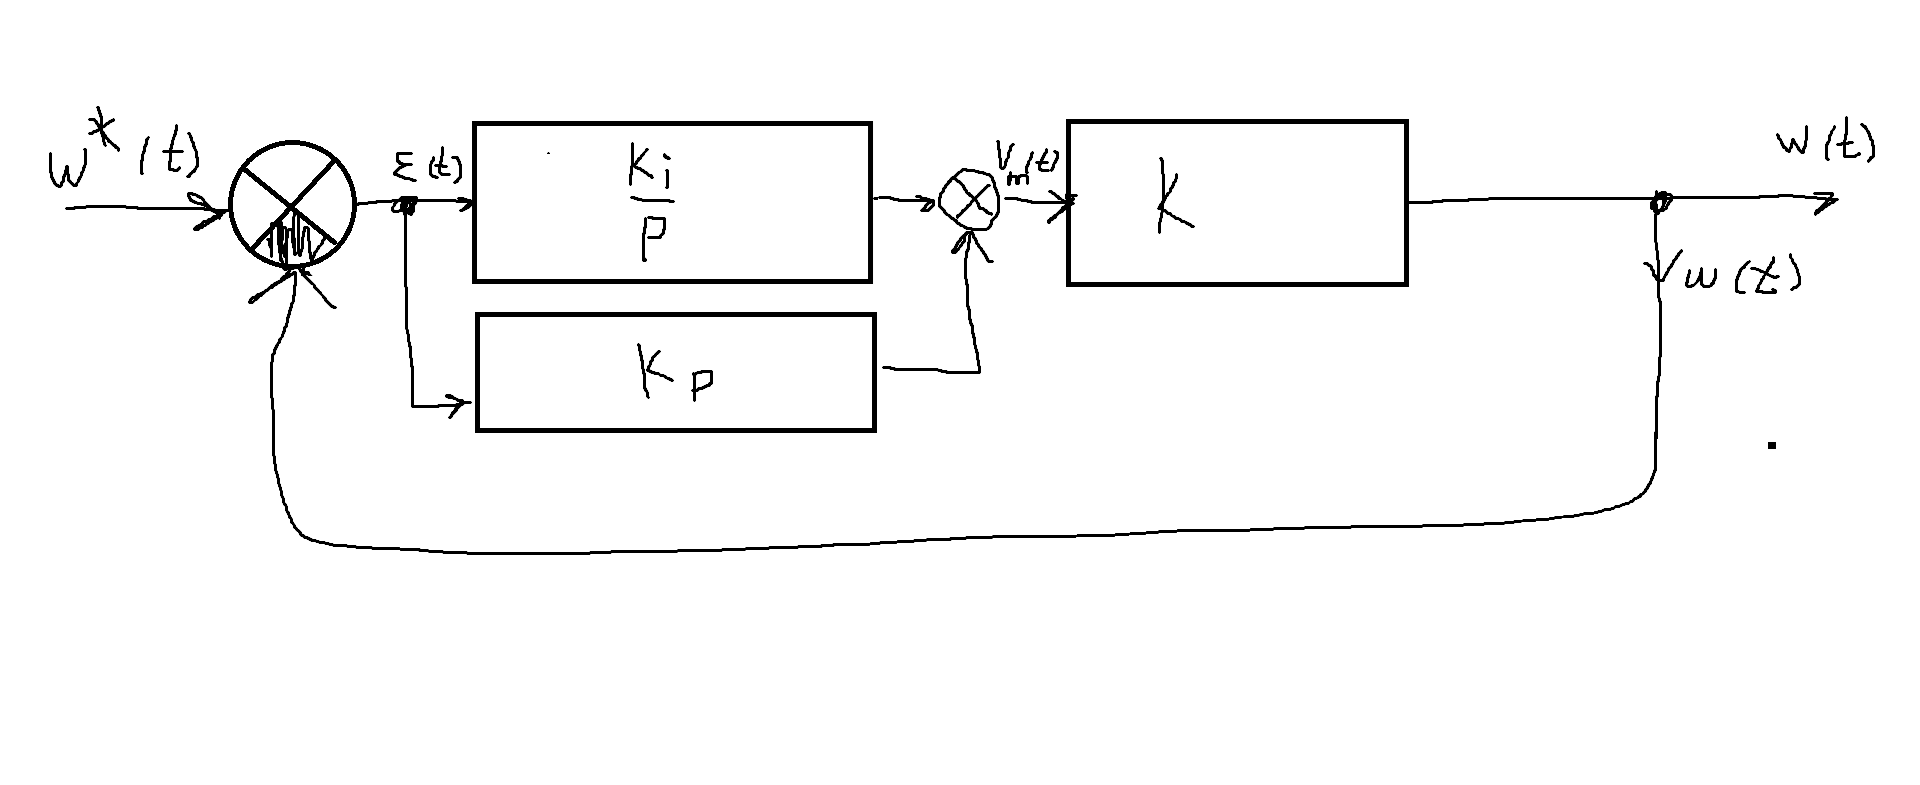
\includegraphics[scale=0.3]{amplifier_and_integrator.png}
		\caption{\label{fig:amplifier_and_integrator}Диграмма пропорционально-интегрального регулятора}
	\end{figure}
	
	Коэффициент передачи такого пропорционально-интегрального регулятора \\ $K_{ai}=...$ \\
	Todo:
	1. Получить коэффициент передачи
	3. Оценить устойчивость, точность (через p=0). Оценить отсутствие ошибки, развернув звено относительно ошибки, подставить в полученный коэффициент p=0.
	2. Для наилучшего типа корней (подставить параметры) интегрирующего звена построить коэффициент передачи, получить переходную функцию в оригиналах (если не получается аналитически, получить численно в следующей главе).
	
	\section{Численные эксперименты построенной математической модели}
	В этой секции нужно подставить в звено коэффициенты из методички и посмотреть на красивые графики выхода на рабочий режим. Оценить макс. отклонение от рабочего режима вверх, время вхождения в рабочий режим, есть ли перерегулирования.
	Очень хорошим опытом будет взять коэффициент как есть, с коэффициентами, и запустить численное интегрирование (обратное преобразование Лаппласа), получив переходную функцию для любых значений коэффициентов. Так мы избежим аналитики. Для функций с разными параметрами можно оценить также величину максимума, количество перерегулирований и время выхода (в т.ч. графически вывести на экран. Время выхода, конечно, численно, интегрируя).
	Написать вывод
	
\end{document}
